\documentclass[a4paper,10pt]{report}
\usepackage{amsmath}
\usepackage{amssymb}
\usepackage{amsfonts}
\usepackage{epstopdf}
\usepackage{epsfig}
\usepackage{textcomp}
\usepackage{inputenc}
\usepackage{fontenc}
\usepackage{graphicx}
\usepackage{color}
\usepackage{breqn}
\usepackage{sectsty}
\usepackage{natbib}
\usepackage{fullpage}
\usepackage{inputenc}
\usepackage{etoolbox}
\usepackage{hyperref}
\usepackage{subfigure}

\begin{document}

\section{Alignments}
\subsection{\# of intermediate controls: 0}
\begin{figure}[!htb]
  \centering
    \subfigure[Basic]
    {
      \centering
        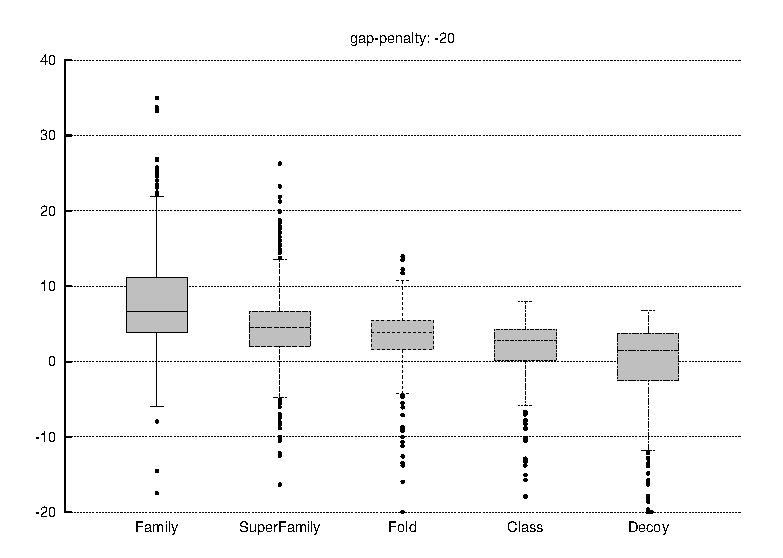
\includegraphics[width=0.45\textwidth]{fig/angles.basic.0.eps}
        \label{fig:angles-basic-0}
    }
    \hspace{0.5cm}
    \subfigure[Affine]
    {
        \centering
        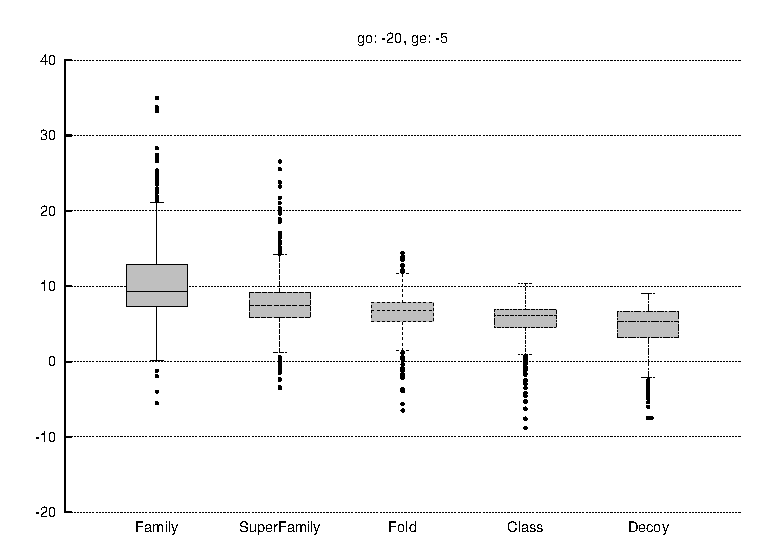
\includegraphics[width=0.45\textwidth]{fig/angles.affine.0.eps}
        \label{fig:angles-affine-0}
    }
    \caption{Alignment of angles only}
    \label{fig:angles-0}
\end{figure}

\subsection{\# of intermediate controls: 0}
\begin{figure}[!htb]
  \centering
    \subfigure[Basic]
    {
      \centering
        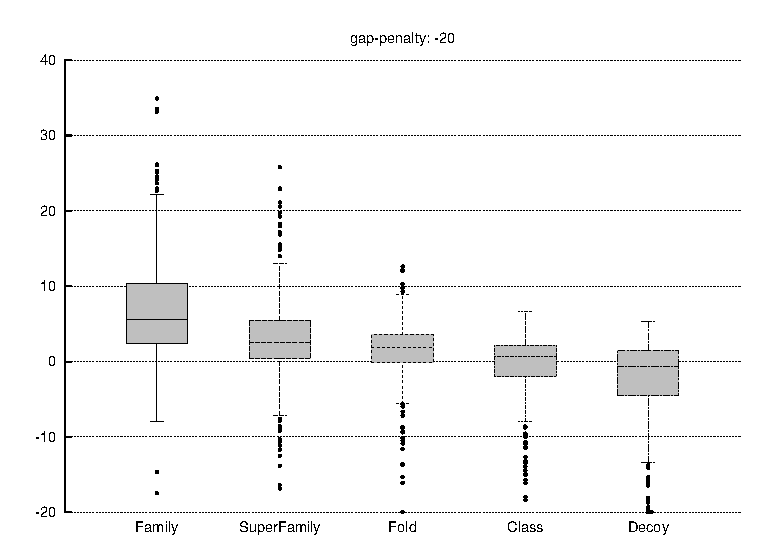
\includegraphics[width=0.45\textwidth]{fig/angles-lengths.basic.0.eps}
        \label{fig:angles-lengths-basic-0}
    }
    \hspace{0.5cm}
    \subfigure[Affine]
    {
        \centering
        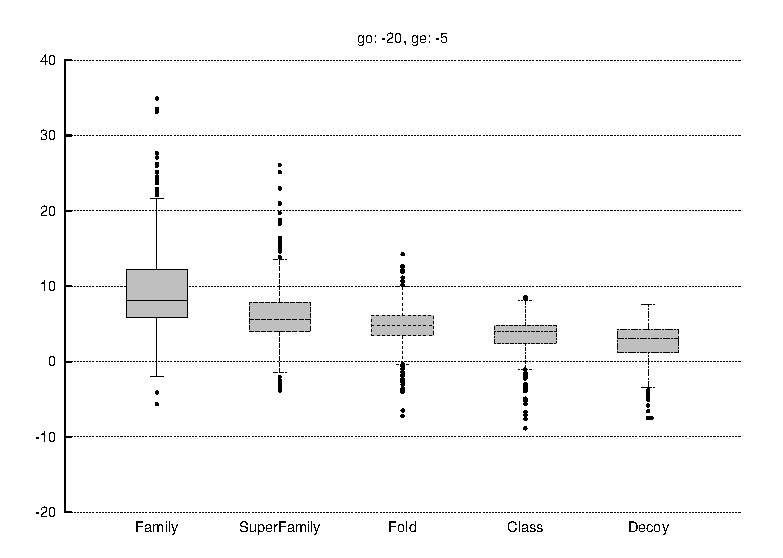
\includegraphics[width=0.45\textwidth]{fig/angles-lengths.affine.0.eps}
        \label{fig:angles-lengths-affine-0}
    }
    \caption{Alignment of angles and lengths}
    \label{fig:angles-lengths-0}
\end{figure}

\newpage

\subsection{\# of intermediate controls: 012}
\begin{figure}[!htb]
  \centering
    \subfigure[Basic]
    {
      \centering
        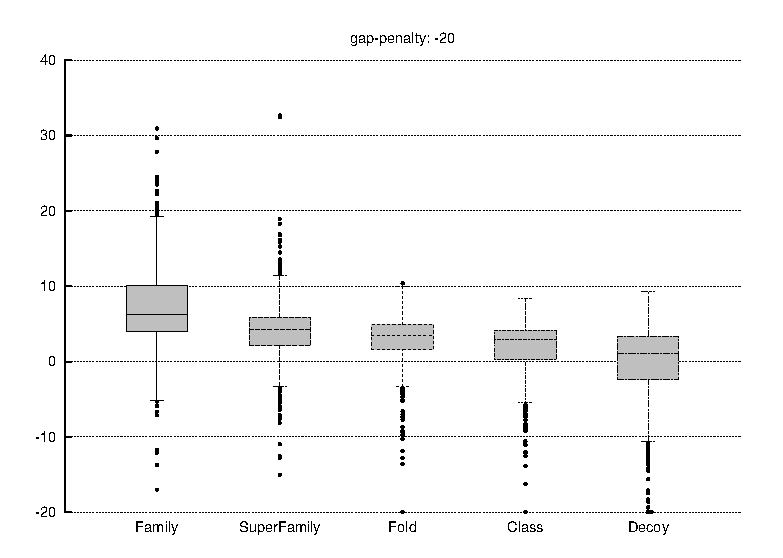
\includegraphics[width=0.45\textwidth]{fig/angles.basic.012.eps}
        \label{fig:angles-basic-012}
    }
    \hspace{0.5cm}
    \subfigure[Affine]
    {
        \centering
        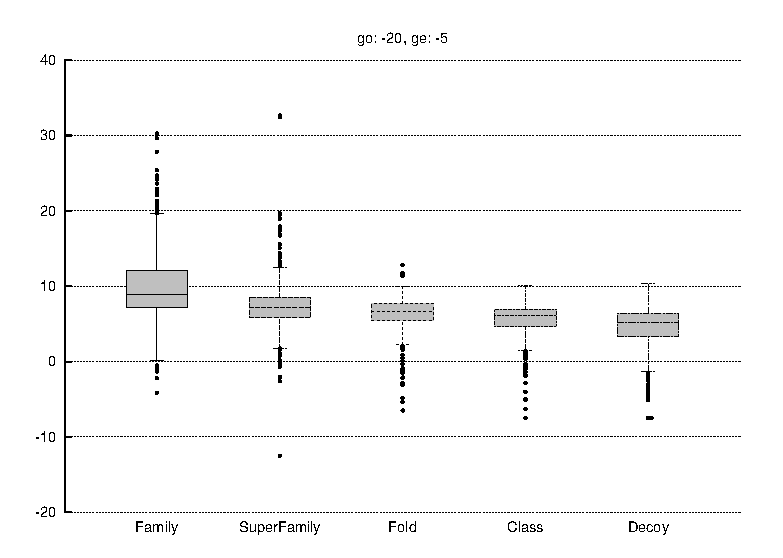
\includegraphics[width=0.45\textwidth]{fig/angles.affine.012.eps}
        \label{fig:angles-affine-012}
    }
    \caption{Alignment of angles only}
    \label{fig:angles-012}
\end{figure}

\subsection{\# of intermediate controls: 012}
\begin{figure}[!htb]
  \centering
    \subfigure[Basic]
    {
      \centering
        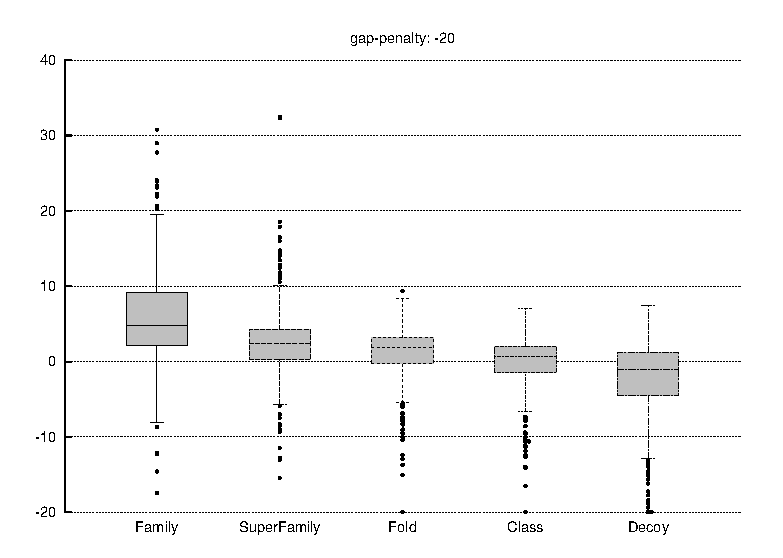
\includegraphics[width=0.45\textwidth]{fig/angles-lengths.basic.012.eps}
        \label{fig:angles-lengths-basic-012}
    }
    \hspace{0.5cm}
    \subfigure[Affine]
    {
        \centering
        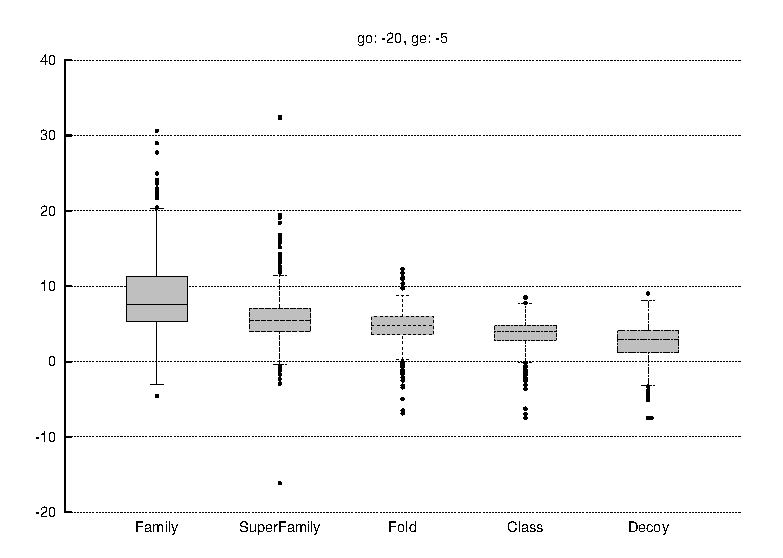
\includegraphics[width=0.45\textwidth]{fig/angles-lengths.affine.012.eps}
        \label{fig:angles-lengths-affine-012}
    }
    \caption{Alignment of angles and lengths}
    \label{fig:angles-lengths-012}
\end{figure}

\newpage

\subsection{SST}
\begin{figure}[!htb]
  \centering
    \subfigure[Basic]
    {
      \centering
        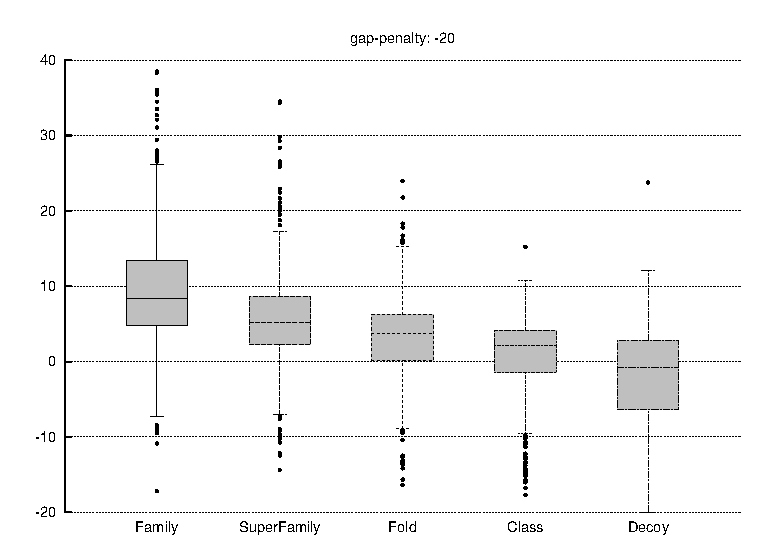
\includegraphics[width=0.45\textwidth]{fig/sst.angles.basic.eps}
        \label{fig:sst-angles-basic}
    }
    \hspace{0.5cm}
    \subfigure[Affine]
    {
        \centering
        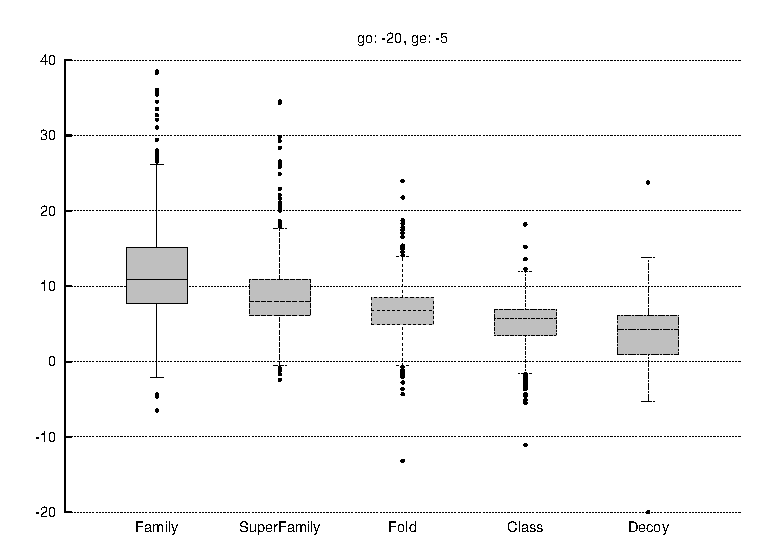
\includegraphics[width=0.45\textwidth]{fig/sst.angles.affine.eps}
        \label{fig:sst-angles-affine}
    }
    \caption{Alignment of angles only}
    \label{fig:sst-angles}
\end{figure}

\subsection{DALI}
\begin{figure}[!htb]
  \centering
  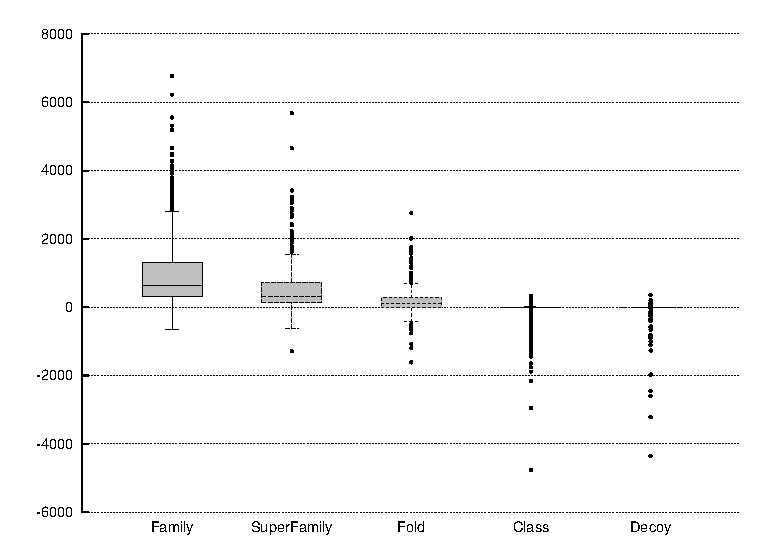
\includegraphics[width=0.45\textwidth]{fig/dali.eps}
  \label{fig:dali}
  \caption{DALI alignment scores}
\end{figure}

\end{document}

